\documentclass[9pt]{beamer}
\usepackage[utf8]{vietnam}
%----------Packages----------
\usepackage{enumitem}
\usepackage{amsmath}
\usepackage{amssymb}
\usepackage{framed,color}
\usepackage{esint}
\usepackage{amsthm}
%\usepackage{amsrefs}
\usepackage{dsfont}
\usepackage{color}
\usepackage{caption}
\usepackage{subcaption}
\usepackage[all]{xy}
\usepackage[mathscr]{eucal}
\usepackage{verbatim}  %%includes comment environmenthttps://www.overleaf.com/7333733538cgxrxfpzqxhk
\usepackage{hyperref}
\usepackage[scr]{rsfso}
\usepackage{tikz}
\usepackage{tikz-cd}
\usepackage{graphicx}

\usepackage[
backend=biber,
style=alphabetic,
sorting=ynt
]{biblatex}
\addbibresource{references.bib}


%---------math operators------
\newcommand{\norm}[1]{\left\lVert#1\right\rVert}
\DeclareMathOperator\supp{supp}
\DeclareMathOperator{\Hom}{Hom}
\DeclareMathOperator{\sets}{\mathbf{Sets}}
\DeclareMathOperator{\topbf}{\mathbf{Top}}
\DeclareMathOperator{\topbfast}{\mathbf{Top_\ast}}
\DeclareMathOperator{\grp}{\mathbf{Groups}}
\DeclareMathOperator{\obj}{obj}
\DeclareMathOperator{\id}{Id}
\DeclareMathOperator{\esssup}{esssup}
\DeclareMathOperator{\sgn}{sgn}

\mode<presentation>
{
  \usetheme{Warsaw}      % or try Darmstadt, Madrid, Warsaw, ...
  \usecolortheme{whale} % or try albatross, beaver, crane, ...
  \usefonttheme{default}  % or try serif, structurebold, ...
  \setbeamertemplate{navigation symbols}{}
  \setbeamertemplate{caption}[numbered]
}

\usepackage[english]{babel}
\usepackage[utf8x]{inputenc}

\numberwithin{equation}{section}

\title[Giải tích sai phân hữu hạn]{Bài Giữa kỳ môn Giải tích sai phân hữu hạn}
\author{Đỗ Sỹ Hưng}
\institute{Trường Đại học Khoa học Tự nhiên, ĐHQG TP.HCM}
\date{Ngày 20 tháng 11 năm 2022}


\begin{document}

\begin{frame}
  \titlepage
\end{frame}

\begin{frame}[allowframebreaks]{Mục lục}
    \tableofcontents[sections={1-2}]
    \framebreak
    \tableofcontents[sections={3-4}]
\end{frame}

\section{Phương pháp giải nghiệm chính xác}

\begin{frame}{Mục lục}
    \tableofcontents[currentsection, sections={1-2}]
\end{frame}

\subsection{Phương trình vi phân}

\begin{frame}
\begin{block}{Bài toán}
    Tìm nghiệm tổng quát của phương trình vi phân sau
    \begin{align}
        u''(x) - 3u'(x) + 2u(x) = 2x^3 - 9x^2 - 2x + 12. \label{pdeq:sample}
    \end{align}
\end{block}
\begin{exampleblock}{Bài giải}
    Phương trình (\ref{pdeq:sample}) là phương trình vi phân tuyến tính cấp 2 không thuần nhất. Nghiệm của phương trình (\ref{pdeq:sample}) có dạng
    \begin{align*}
        u(x) = u_h(x) + u_p(x),
    \end{align*}
    trong đó $u_p$ là một nghiệm cụ thể của phương trình (\ref{pdeq:sample}), $u_h$ là nghiệm của phương trình tuyến tính cấp 2 thuần nhất
    \begin{align}
        u''(x) - 3u'(x) + 2u(x) = 0. \label{pdeq:homo_sample}
    \end{align}
    Xét phương trình đặc trưng của phương trình (\ref{pdeq:homo_sample}), chúng ta được
    \begin{align*}
        \lambda^2 - 3\lambda + 2 = 0
    \end{align*}
\end{exampleblock}
\end{frame}

\begin{frame}
\begin{exampleblock}{Bài giải}
    Phương trình đặc trưng có hai nghiệm $\lambda = 1$ và $\lambda = 2$, tương ứng với nghiệm
    \begin{align*}
        u_h(x) = C_1 e^x + C_2 e^{2x}
    \end{align*}
    với $C_1$, $C_2$ là hai hằng số tùy ý. \\
    Vì $u_p$ là một nghiệm của phương trình (\ref{pdeq:sample}), bằng phương pháp hệ số bất định, nghiệm $u_p$ có dạng
    \begin{align*}
        u_p(x) = Ax^3 + Bx^2 + Cx + D.
    \end{align*}
    Đạo hàm cấp một và cấp hai tương ứng của nghiệm $u_p$ là
    \begin{align*}
        u_p'(x) &= 3Ax^2 + 2Bx + C, \\
        u_p''(x) &= 6Ax + 2B.
    \end{align*}
\end{exampleblock}

\end{frame}
\begin{frame}
\begin{exampleblock}{Bài giải}
     Khi đó,
    \begin{align*}
        &u_p''(x) - 3u_p'(x) + 2u_p \\
        &\quad = (6Ax + 2B) - 3(3Ax^2 + 2Bx + C) + 2(Ax^3 + Bx^2 + Cx + D) \\
        &\quad = 2Ax^3 + (-9A + 2B)x^2 + (6A - 6B + 2C)x + 2B - 3C + 2D.    
    \end{align*}
    Đồng nhất hệ số hai vế của đẳng thức
    \begin{align*}
        u_p''(x) - 3u_p'(x) + 2u_p(x) = 2x^3 - 9x^2 - 2x + 12.
    \end{align*}
    Ta được hệ phương trình
    \begin{align*}
        \begin{cases}
        2A &= 2 \\
        -9A + 2B &= -9 \\
        6A - 6B + 2C &= -2 \\
        2B - 3C + 2D &= 12
        \end{cases} \Leftrightarrow
        \begin{cases}
        A &= 1, \\
        B &= 0, \\
        C &= -4, \\
        D &= 0.
        \end{cases}
    \end{align*}
\end{exampleblock}
\end{frame}

\begin{frame}
\begin{exampleblock}{Bài giải}
     Khi đó, nghiệm riêng $u_p$ là
    \begin{align*}
        u_p(x) = x^3 - 4x.
    \end{align*}
    Nghiệm tổng quát của phương trình (\ref{pdeq:sample}) là
    \begin{align}
        u(x) &= u_h(x) + u_p(x) \nonumber \\
        u(x) &= C_1 e^x + C_2 e^{2x} + x^3 - 4x. \label{pdeq:solution}
    \end{align}
    Đạo hàm của $u$ là
    \begin{align}
        u'(x) = C_1 e^x + 2C_2 e^{2x} + 3x^2 - 4. \label{pdeq:deri}
    \end{align} \hfill \qed
\end{exampleblock}
\end{frame}

\subsection{Điều kiện biên Dirichlet}

\begin{frame}
\begin{block}{Bài toán điều kiện biên Dirichlet}
    Tìm nghiệm chính xác của phương trình vi phân
    \begin{align*}
        \begin{cases}
        u''(x) - 3u'(x) + 2u(x) = 2x^3 - 9x^2 - 2x + 12, \\
        u(-1) = 3, \ u(2) = 0.
        \end{cases}
    \end{align*}
\end{block}
\begin{exampleblock}{Bài giải}
    Thế điều kiện biên Dirichet $u(-1) = 3$, $u(2) = 0$ vào nghiệm tổng quát (\ref{pdeq:solution}), ta được hệ phương trình
    \begin{align*}
        \begin{cases}
        C_1 e^{-1} + C_2 e^{-2} + 3 &= 3 \\
        C_1 e^2 + C_2 e^4 &= 0
        \end{cases} \Leftrightarrow
        \begin{cases}
        C_1 e^{-1} + C_2 e^{-2} &= 0 \\
        C_1 e^2 + C_2 e^4 &= 0
        \end{cases} \Leftrightarrow
    C_1 = C_2 = 0.
    \end{align*}
    Nghiệm riêng của phương trình là
    \begin{align*}
        u(x) = x^3 - 4x.
    \end{align*} \hfill \qed
\end{exampleblock}
\end{frame}

\subsection{Điều kiện biên Neuman và Dirichlet}

\begin{frame}
\begin{block}{Bài toán điều kiện biên Neuman và Dirichlet}
    Tìm nghiệm chính xác của phương trình vi phân
    \begin{align*}
        \begin{cases}
        u''(x) - 3u'(x) + 2u(x) = 2x^3 - 9x^2 - 2x + 12, \\
        u'(-1) = -1, \ u(2) = 0.
        \end{cases}
    \end{align*}
\end{block}
\begin{exampleblock}{Bài giải}
    Thế điều kiện biên Neuman $u'(-1) = -1$ vào (\ref{pdeq:deri}), và điều kiện Dirichlet $u(2) = 0$ vào (\ref{pdeq:solution}), ta được hệ phương trình
    \begin{align*}
        \begin{cases}
        C_1 e^{-1} + 2C_2 e^{-2} - 1 &= -1 \\
        C_2 e^2 + C_2 e^4 &= 0
        \end{cases} \Leftrightarrow
        \begin{cases}
        C_1 e^{-1} + 2C_2 e^{-2} &= 0 \\
        C_2 e^2 + C_2 e^4 &= 0
        \end{cases} \Leftrightarrow
        C_1 = C_2 = 0.
    \end{align*}
    Nghiệm riêng của phương trình là
    \begin{align*}
        u(x) = x^3 - 4x.
    \end{align*} \hfill \qed
\end{exampleblock}
\end{frame}

\subsection{Điều kiện biên Robin và Neuman}

\begin{frame}
\begin{block}{Bài toán điều kiện biên Robin và điều kiện Neuman}
    Tìm nghiệm chính xác của phương trình vi phân
    \begin{align*}
        \begin{cases}
        u''(x) - 3u'(x) + 2u(x) = 2x^3 - 9x^2 - 2x + 12, \\
        u(-1) + u'(-1) = 2, \ u'(2) = 8.
        \end{cases} 
    \end{align*}
\end{block}
\begin{exampleblock}{Bài giải}
    Thế điều kiện biên Robin $u'(-1) + u(-1) = 2$ vào (\ref{pdeq:solution}), (\ref{pdeq:deri}), và điều kiện Neuman $u'(2) = 8$ vào (\ref{pdeq:deri}), ta được hệ phương trình
    \begin{align*}
        &\begin{cases}
        (C_1 e^{-1} + C_2 e^{-2} + 3) + (C_1 e^{-1} + 2C_2 e^{-2} - 1) &= 2 \\
        C_2 e^2 + 2C_2 e^4 +8 &= 8
        \end{cases} \\
        &\Leftrightarrow
        \begin{cases}
        2C_1 e^{-1} + 3C_2 e^{-2} + 2 &= 2 \\
        C_2 e^2 + 2C_2 e^4 &= 0
        \end{cases} \Leftrightarrow
        \begin{cases}
        2C_1 e^{-1} + 3C_2 e^{-2} &= 0 \\
        C_2 e^2 + C_2 e^4 &= 0
        \end{cases} \Leftrightarrow
        \begin{cases}
        C_1 &= 0, \\ C_2 &= 0.
        \end{cases}
    \end{align*}
    Nghiệm riêng của phương trình là $u(x) = x^3 - 4x.$ \hfill \qed
\end{exampleblock}
\end{frame}

\subsection{Điều kiện biên Robin}

\begin{frame}
\begin{block}{Bài toán điều kiện biên Robin}
    Tìm nghiệm chính xác của phương trình vi phân
    \begin{align*}
        \begin{cases}
        u''(x) - 3u'(x) + 2u(x) = 2x^3 - 9x^2 - 2x + 12, \\
        u(-1) + u'(-1) = 2, \ u(2) + u'(2) = 8.
        \end{cases}
    \end{align*}
\end{block}
\begin{exampleblock}{Bài giải}
    Thế các điều kiện biên Robin $u'(-1) + u(-1) = 2$, $u'(2) + u(2) = 8$ vào (\ref{pdeq:solution}), (\ref{pdeq:deri}), ta được hệ phương trình
    \begin{align*}
        &\begin{cases}
        (C_1 e^{-1} + C_2 e^{-2} + 3) + (C_1 e^{-1} + 2C_2 e^{-2} - 1) &= 2 \\
        (C_1 e^2 + C_2 e^4) + (C_2 e^2 + 2C_2 e^4 + 8) &= 8
        \end{cases} \\
        &\Leftrightarrow
        \begin{cases}
        2C_1 e^{-1} + 3C_2 e^{-2} + 2 &= 2 \\
        2C_2 e^2 + 3C_2 e^4 + 8 &= 8
        \end{cases} \Leftrightarrow
        \begin{cases}
        2C_1 e^{-1} + 3C_2 e^{-2} &= 0 \\
        2C_2 e^2 + 3C_2 e^4 &= 0
        \end{cases} \Leftrightarrow
        \begin{cases}
        C_1 &= 0, \\ C_2 &= 0.
        \end{cases}
    \end{align*}
    Nghiệm riêng của phương trình là $u(x) = x^3 - 4x.$ \hfill \qed
\end{exampleblock}
\end{frame}

\section{Phương pháp sai phân hữu hạn}

\begin{frame}{Mục lục}
    \tableofcontents[currentsection, sections={1-2}]
\end{frame}

\subsection{Phương pháp sai phân hữu hạn tổng quát}

\begin{frame}
\begin{block}{Bài toán}
    Giải phương trình vi phân bằng phương pháp sai phân hữu hạn
    \begin{equation}
        u''(x) + \alpha u'(x) + \beta u(x) = f(x), \ x \in (a,b), \label{deq:sample}
    \end{equation}
    với $\alpha$, $\beta$ là các hằng số thực, hàm $f$ là hàm ngoại lực.
\end{block}
    
\begin{exampleblock}{Bài giải}
    Ta chia lưới đều trên đoạn $(a,b)$ thành $a = x_1 \le x_2 \le \ldots \le x_n = b$. Đặt $h = x_2 - x_1 $. Gọi $u_1, u_2, \ldots, u_n$ lần lượt là các giá trị xấp xỉ của $u(x_1), u(x_2), \ldots, u(x_n)$, .Khi đó với mỗi giá trị $i = \overline{2, n-1}$, thực hiện xấp xỉ đạo hàm cấp một $u'(x_i)$ và cấp hai $u''(x_i)$ như sau
    \begin{align*}
        u'(x_i) &\approx \frac{u_{i+1} - u_{i-1}}{2h} + O(h^2), \\
        u''(x_i) &\approx \frac{u_{i-1} - 2u_i + u_{i+1}}{h^2} + O(h^2).
    \end{align*}
\end{exampleblock}
\end{frame}

\begin{frame}
\begin{exampleblock}{Bài giải}
    Thế giá trị xấp xỉ $u'(x_i)$ và $u''(x_i)$ vào phương trình vi phân (\ref{deq:sample}), ta được
    \begin{align*}
        \frac{u_{i-1} - 2u_i + u_{i+1}}{h^2} + \alpha \frac{u_{i+1} - u_{i-1}}{2h} + \beta u_i = f(x_i)
    \end{align*}
    Rút các hệ số của $u_{i-1}$, $u_i$ và $u_{i+1}$
    \begin{align*}
        \left(\frac{1}{h^2} - \frac{\alpha}{2h}\right) u_{i-1} + \left(-\frac{2}{h^2}+\beta\right) u_i + \left(\frac{1}{h^2} + \frac{\alpha}{2h}\right) u_{i+1} = f(x_i)
    \end{align*}
    Nhân hai vế cho $2h^2$
    \begin{align}
        (2 - \alpha h) u_{i-1} + (-4 + 2\beta h^2) u_i + (2 + \alpha h) u_{i+1} = 2h^2 f(x_i) \label{deq:solution}
    \end{align}
\end{exampleblock}
\end{frame}

\begin{frame}
\begin{exampleblock}{Bài giải}
    Khi đó, ta được công thức ma trận, không có điều kiện biên, ${\bf M} {\bf u} = {\bf B}$, với ma trận ${\bf M}$ là
    \begin{align*}
        \begin{pmatrix}
            \dots & \dots & \dots & \dots & \dots & \dots & \dots & \dots \\
            2 - \alpha h & -4 + 2\beta h^2 & 2 + \alpha h & 0 & \dots & 0 & 0 & 0 \\
            0 & 2 - \alpha h & -4 + 2\beta h^2 & 2 + \alpha h & \dots & 0 & 0 & 0 \\
            \vdots & \vdots & \vdots & \vdots & \ddots & \vdots & \vdots & \vdots \\
            0 & 0 & 0 & 0 & \dots & 2 - \alpha h & -4 + 2\beta h^2 & 2 + \alpha h \\
            \dots & \dots & \dots & \dots & \dots & \dots & \dots & \dots
        \end{pmatrix}
    \end{align*}
    và hai vector cột ${\bf u}$, ${\bf B}$ là
    \begin{align*}
        {\bf u} &= (u_1, u_2, \ldots, u_n)^T, \\
        {\bf B} &= (b_1, 2h^2 f(x_2), 2h^2 f(x_3), \dots, 2h^2 f(x_{n-1}), b_n)^T.
    \end{align*}
    với $b_1, b_n$ là hai giá trị phụ thuộc điều kiện biên. \fhill \qed
\end{exampleblock}
\end{frame}

\subsection{Phương pháp SPHH cho điều kiện Dirichlet}

\begin{frame}
\begin{block}{Bài toán điều kiện biên Dirichlet}
    Giải phương trình vi phân bằng phương pháp sai phân hữu hạn
    \begin{align*}
        \begin{cases}
        u''(x) + \alpha u'(x) + \beta u(x) = f(x), \ x \in (a,b), \\
        u(a) = D_a, u(b) = D_b.
        \end{cases}
    \end{align*}
    với $\alpha$, $\beta$ là các hằng số thực, hàm $f$ là hàm ngoại lực.
\end{block}

\begin{exampleblock}{Bài giải}
    Từ điều kiện biên Dirichlet $u(a) = D_a$, $u(b) = D_b$, công thức ma trận cho bài toán có dạng
    \begin{align*}
        \begin{pmatrix}
            1 & 0 & \dots & 0 & 0 \\
            \vdots & \vdots & \vdots & \ddots & \vdots \\
            0 & 0 & \dots & 0 & 1
        \end{pmatrix}
        \begin{pmatrix}
            u_1 \\ \vdots \\ u_n
        \end{pmatrix} =
        \begin{pmatrix}
            D_a \\ \vdots \\ D_b
        \end{pmatrix}.
    \end{align*} \hfill \qed
\end{exampleblock}
\end{frame}

\subsection{Phương pháp SPHH cho điều kiện biên Neuman}

\begin{frame}
\begin{block}{Bài toán điều kiện biên Neuman bên trái}
    Giải phương trình vi phân bằng phương pháp sai phân hữu hạn
    \begin{align*}
        \begin{cases}
        u''(x) + \alpha u'(x) + \beta u(x) = f(x), \ x \in (a,b), \\
        u'(a) = N_a.
        \end{cases}
    \end{align*}
    với $\alpha$, $\beta$ là các hằng số thực, hàm $f$ là hàm ngoại lực.
\end{block}

\begin{exampleblock}{Bài giải}
    Xét tại $i = 1$, ta thêm một điểm ảo $x_0$ (ghost point) về phía bên trái đoạn $(a,b)$, thỏa $x_1 - x_0 = h$, khi đó
    \begin{align*}
        u'(x_1) \approx \frac{u(x_2) - u(x_0)}{2h}.
    \end{align*}
    Thực hiện xấp xỉ $u(x_i)$ bằng các giá trị $u_i$ cho điều kiện biên Neuman
    \begin{align*}
        N_a = \frac{u_2 - u_0}{2h} \Leftrightarrow u_0 = u_2 - 2h N_a.
    \end{align*}
\end{exampleblock}
\end{frame}

\begin{frame}
\begin{exampleblock}{Bài giải}
    Tại $i = 1$, (\ref{deq:solution}) trở thành
    \begin{align}
        (2 - \alpha h) u_0 + (-4 + 2\beta h^2) u_1 + (2 + \alpha h) u_2 = 2h^2 f(x_1). \label{deq:nleft}
    \end{align}
    Thế $u_0$ vào (\ref{deq:nleft}), ta được
    \begin{align*}
        (2 - \alpha h) (u_2 - 2h N_a) + (-4 + 2\beta h^2) u_1 + (2 + \alpha h) u_2 = 2h^2 f(x_1).
    \end{align*}
    Rút các hệ số của $u_1$ và $u_2$
    \begin{align}
        (-4 + 2\beta h^2) u_1 + 4 u_2 = 2h^2 f(x_1) + 2hN_a(2 - \alpha h). \label{deq:nl_solution}
    \end{align}
\end{exampleblock}
\end{frame}

\begin{frame}
\begin{exampleblock}{Bài giải}
    Từ (\ref{deq:nl_solution}), công thức ma trận ${\bf M} {\bf u} = {\bf B}$ trong đó
    \begin{align*}
        {\bf M} &= \begin{pmatrix}
            -4 + 2\beta h^2 & 4 & 0 & \dots & 0 \\
            \vdots & \vdots & \vdots & \vdots & \vdots
        \end{pmatrix}, \\
        {\bf u} &= (u_1, u_2, \dots, u_n)^T, \\
        {\bf B} &= \begin{pmatrix}
            2h^2 f(x_1) + 2h N_a (2 - \alpha h) \\
            \vdots
        \end{pmatrix}
    \end{align*} \hfill \qed
\end{exampleblock}
\end{frame}

\begin{frame}
\begin{block}{Bài toán điều kiện biên Neuman bên phải}
    Giải phương trình vi phân bằng phương pháp sai phân hữu hạn
    \begin{align*}
        \begin{cases}
        u''(x) + \alpha u'(x) + \beta u(x) = f(x), \ x \in (a,b), \\
        u'(b) = N_b.
        \end{cases}
    \end{align*}
    với $\alpha$, $\beta$ là các hằng số thực, hàm $f$ là hàm ngoại lực.
\end{block}

\begin{exampleblock}{Bài giải}
    Xét tại $i = n$, ta thêm một điểm ảo $x_{n+1}$ (ghost point) về phía bên phải đoạn $(a,b)$, thỏa $x_{n+1} - x_n = h$, khi đó
    \begin{align*}
        u'(x_n) \approx \frac{u(x_{n+1}) - u(x_{n-1})}{2h}.
    \end{align*}
    Thực hiện xấp xỉ $u(x_i)$ bằng các giá trị $u_i$ cho điều kiện biên Neuman
    \begin{align*}
        N_b = \frac{u_{n+1} - u_{n-1}}{2h} \Leftrightarrow u_{n+1} = u_{n-1} + 2h N_b.
    \end{align*}
\end{exampleblock}
\end{frame}

\begin{frame}
\begin{exampleblock}{Bài giải}
    Tại $i = n$, (\ref{deq:solution}) trở thành
    \begin{align}
        (2 - \alpha h) u_{n-1} + (-4 + 2\beta h^2) u_n + (2 + \alpha h) u_{n+1} = 2h^2 f(x_n). \label{deq:nright}
    \end{align}
    Thế $u_{n+1}$ vào (\ref{deq:nright}), ta được
    \begin{align*}
        (2 - \alpha h) u_{n-1} + (-4 + 2\beta h^2) u_n + (2 + \alpha h) (u_{n-1} + 2h N_b) = 2h^2 f(x_n).
    \end{align*}
    Rút các hệ số của $u_{n-1}$ và $u_n$
    \begin{align}
        4 u_{n-1} + (-4 + 2\beta h^2) u_n = 2h^2 f(x_n) - 2h N_b (2 + \alpha h). \label{deq:nr_solution}
    \end{align}
\end{exampleblock}
\end{frame}

\begin{frame}
\begin{exampleblock}{Bài giải}
    Từ (\ref{deq:nr_solution}), công thức ma trận ${\bf M} {\bf u} = {\bf B}$ trong đó
    \begin{align*}
        {\bf M} &= \begin{pmatrix}
            \vdots & \vdots & \vdots & \vdots & \vdots \\
            4 & -4 + 2\beta h^2 & 0 & \dots & 0
        \end{pmatrix}, \\
        {\bf u} &= (u_1, u_2, \dots, u_n)^T, \\
        {\bf B} &= \begin{pmatrix}
            \vdots \\
            2h^2 f(x_n) - 2h N_b (2 + \alpha h)
        \end{pmatrix}
    \end{align*} \hfill \qed
\end{exampleblock}
\end{frame}

\subsection{Phương pháp SPHH cho điều kiện biên Robin}

\begin{frame}
\begin{block}{Bài toán điều kiện biên Robin bên trái}
    Giải phương trình vi phân bằng phương pháp sai phân hữu hạn
    \begin{align*}
        \begin{cases}
        u''(x) + \alpha u'(x) + \beta u(x) = f(x), \ x \in (a,b), \\
        C_a u'(a) + D_a u(a) = R_a.
        \end{cases}
    \end{align*}
    với $\alpha$, $\beta$ là các hằng số thực, hàm $f$ là hàm ngoại lực.
\end{block}

\begin{exampleblock}{Bài giải}
    Xét tại $i = 1$, ta thêm một điểm ảo $x_0$ (ghost point) vào phía bên trái đoạn $(a,b)$, thỏa $x_1 - x_0 = h$, khi đó
    \begin{align*}
        u'(x_1) \approx \frac{u(x_2) - u(x_0)}{2h}.
    \end{align*}
    Thực hiện xấp xỉ $u(x_i)$ bằng các giá trị $u_i$ cho điều kiện biên Robin
    \begin{align*}
        C_a \frac{u_2 - u_0}{2h} + D_b u_1 = R_a
        \Leftrightarrow u_0 = u_2 - \frac{2h}{C_a}(R_a - D_a u_1).
    \end{align*}
\end{exampleblock}
\end{frame}

\begin{frame}
\begin{exampleblock}{Bài giải}
    Tại $i = 1$, (\ref{deq:solution}) trở thành
    \begin{align}
        (2 - \alpha h) u_0 + (-4 + 2\beta h^2) u_1 + (2 + \alpha h) u_2 = 2h^2 f(x_1). \label{deq:rleft}
    \end{align}
    Thế $u_0$ vào phương trình (\ref{deq:rleft}), ta được
    \begin{align*}
        (2 - \alpha h) \left(u_2 - \frac{2h}{C_a}(R_a - D_a u_1)\right) + (-4 + 2\beta h^2) u_1 + (2 + \alpha h) u_2 = 2h^2 f(x_1).
    \end{align*}
    Rút các hệ số $u_1$ và $u_2$
    \begin{align}
        \left(2h \frac{D_a}{C_a} (2 - \alpha h) - 4 + 2\beta h^2\right) u_1 + 4u_2 = 2h^2 f(x_1) + 2h \frac{R_a}{C_a} (2 + \alpha h). \label{deq:rl_solution}
    \end{align}
\end{exampleblock}
\end{frame}

\begin{frame}
\begin{exampleblock}{Bài giải}
    Từ (\ref{deq:rl_solution}), công thức ma trận ${\bf M} {\bf u} = {\bf B}$ trong đó
    \begin{align*}
        {\bf M} &= \begin{pmatrix}
            2h \frac{D_a}{C_a}(2 - \alpha h) - 4 + 2\beta h^2 & 4 & 0 & \dots & 0 \\
            \vdots & \vdots & \vdots & \vdots & \vdots
        \end{pmatrix}, \\
        {\bf u} &= (u_1, u_2, \ldots, u_n)^T, \\
        {\bf B} &= \begin{pmatrix}
            2h^2 f(x_1) + 2h \frac{R_a}{C_a}(2 - \alpha h) \\
            \vdots
        \end{pmatrix}
    \end{align*} \hfill \qed
\end{exampleblock}
\end{frame}

\begin{frame}
\begin{block}{Bài toán điều kiện biên Robin bên phải}
    Giải phương trình vi phân bằng phương pháp sai phân hữu hạn
    \begin{align*}
        \begin{cases}
        u''(x) + \alpha u'(x) + \beta u(x) = f(x), \ x \in (a,b), \\
        C_b u'(b) + D_b u(b) = R_b.
        \end{cases}
    \end{align*}
    với $\alpha$, $\beta$ là các hằng số thực, hàm $f$ là hàm ngoại lực.
\end{block}

\begin{exampleblock}{Bài giải}
    Xét tại $i = n$, ta thêm một điểm ảo $x_{n+1}$ (ghost point) vào phía bên phải đoạn $(a,b)$, thỏa $x_{n+1} - x_n = h$, khi đó
    \begin{align*}
        u'(x_n) \approx \frac{u(x_{n+1}) - u(x_{n-1})}{2h}.
    \end{align*}
    Thực hiện xấp xỉ $u(x_i)$ bằng các giá trị $u_i$ cho điều kiện biên Robin
    \begin{align*}
        C_b \frac{u_{n+1} - u_{n-1}}{2h} + D_b u_n = R_b
        \Leftrightarrow u_{n+1} = u_{n-1} + \frac{2h}{C_b}(R_b - D_b u_n).
    \end{align*}
\end{exampleblock}
\end{frame}

\begin{frame}
\begin{exampleblock}{Bài giải}
    Tại $i = n$, (\ref{deq:solution}) trở thành
    \begin{align}
        (2 - \alpha h) u_{n-1} + (-4 + 2 \beta h^2) u_n + (2 + \alpha h) u_{n+1} = 2h^2 f(x_n). \label{deq:rright}
    \end{align}
    Thế $u_{n+1}$ vào phương trình (\ref{deq:rright}), ta được
    \begin{align*}
        (2 - \alpha h) u_{n-1} + (-4 + 2 \beta h^2) u_n + (2 + \alpha h) \left(u_{n-1} + \frac{2h}{C_b}(R_b - D_b u_n)\right) = 2h^2 f(x_n).
    \end{align*}
    Rút các hệ số của $u_{n-1}$ và $u_{n+1}$
    \begin{align}
        4 u_{n-1} + \left(-4 + 2\beta h^2 -2h \frac{D_b}{C_b}  (2 + \alpha h)\right) u_n = 2h^2 f(x_n) - 2h \frac{R_b}{C_b}(2 + \alpha h). \label{deq:rr_solution}
    \end{align}
\end{exampleblock}
\end{frame}

\begin{frame}
\begin{exampleblock}{Bài giải}
    Từ (\ref{deq:rr_solution}), công thức ma trận ${\bf M} {\bf u} = {\bf B}$ trong đó
    \begin{align*}
        {\bf M} &= \begin{pmatrix}
            \vdots & \vdots & \vdots & \vdots & \vdots & \vdots \\
            0 & 0 & 0 & \dots & 4 & - 4 + 2\beta h^2 - 2h \frac{D_b}{C_b}(2 + \alpha h)
        \end{pmatrix}, \\
        {\bf u} &= (u_1, u_2, \ldots, u_n)^T, \\
        {\bf B} &= \begin{pmatrix}
            \vdots \\
            2h^2 f(x_1) - 2h \frac{R_b}{C_b}(2 + \alpha h)
        \end{pmatrix}
    \end{align*} \hfill \qed
\end{exampleblock}
\end{frame}

\section{Một số bài toán sai phân hữu hạn và đánh giá sai số}

\begin{frame}{Mục lục}
    \tableofcontents[currentsection, sections={3-4}]
\end{frame}

\subsection{Đánh giá sai số và bậc hội tụ}

\begin{frame}
\begin{block}{Định nghĩa Chuẩn (norm)}
    Cho vector ${\bf E} = (e_1,\ldots,e_n) \in \mathbb{R}^n$, khi đó ta định nghĩa các chuẩn của ${\bf E}$ như sau
    \begin{itemize}
        \item \textbf{Chuẩn max}: $\|E\|_{\infty} = \max_{i = 1 \ldots n} \{|e_i|\}$,
        \item \textbf{Chuẩn 1}: $\|E\|_1 = \sum_{i=1}^n h_i |e_i|$,
        \item \textbf{Chuẩn 2}: $\|E\|_2 = \left(\sum_{i=1}^n h_i |e_i|^2\right)^{1/2}$,
    \end{itemize}
    với $h_i = x_{i+1} - x_i$.
\end{block}

\begin{block}{Định nghĩa Sai số toàn cục (Global error)}
    Cho lưới $x_1,\ldots,x_n$, vector ${\bf u} = (u_1,\ldots u_n)$ là nghiệm chính xác và vector ${\bf U} = (U_1,\ldots,U_n)$ là nghiệm xấp xỉ bằng Phương pháp sai phân. Khi đó vector
    \begin{align*}
        E = U - u
    \end{align*}
    được gọi là \textbf{Sai số toàn cục}.
\end{block}
\end{frame}

\begin{frame}
\begin{block}{Định nghĩa Bậc hội tụ}
    Gọi ${\bf E}$ là sai số toàn cục của phương pháp sai phân hữu hạn, nếu ${\bf E}$ thoả mãn bất đẳng thức
    \begin{align*}
        \|{\bf E}\| \le Ch^p, p > 0
    \end{align*}
    thì phương pháp sai phân có \textbf{bậc hội tụ} là $p$.
\end{block}

\begin{exampleblock}{Định lý}
    Gọi ${\bf E_1}, {\bf E_2}$ lần lượt là các sai số toàn cục khi chia lưới gồm $n_1$ điểm và $n_2$ điểm. Bậc hội tụ $p$ của phương pháp sai phân được xấp xỉ bởi công thức
    \begin{align*}
        p \approx - \frac{\log \|{\bf E_1}\| - \log \|{\bf E_2}\|}{\log(n_1) - \log(n_2)}.
    \end{align*}
\end{exampleblock}
\end{frame}

\subsection{Điều kiện biên Dirichlet}

\begin{frame}
\begin{block}{Bài toán điều kiện biên Dirichlet}
    Tìm nghiệm của phương trình vi phân bằng phương pháp sai phân hữu hạn
    \begin{align*}
    \begin{cases}
        u''(x) - 3u'(x) + 2u(x) = 2x^3 - 9x^2 - 2x + 12, \\
        u(-1) = 3, \ u(2) = 0.
    \end{cases}
    \end{align*}
\end{block}
    
\begin{exampleblock}{Bài giải}
    \begin{center}\begin{tabular}{||c|c|c|c||}
    \hline
    n & Sai số tuyệt đối & Sai số tương đối & Bậc hội tụ \\
    \hline\hline
    8   & 1.0434 & 0.3424 & 2.096 \\
    16  & 0.2441 & 0.0800 & 2.020 \\
    32  & 0.0602 & 0.0195 & 2.007 \\
    64  & 0.0150 & 0.0049 & 2.002 \\
    \hline
    \end{tabular}\end{center}
\end{exampleblock}
\end{frame}

\begin{frame}
\begin{exampleblock}{Bài giải}
    \begin{center}
        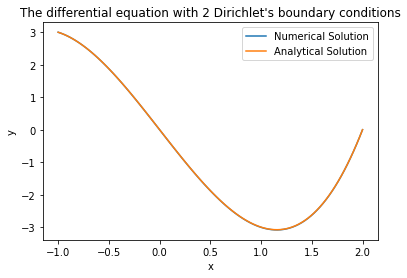
\includegraphics[scale=0.5]{img/midterm1}
    \end{center}
    \qed
\end{exampleblock} 
\end{frame}

\subsection{Điều kiện biên Neuman và Dirichlet}

\begin{frame}
\begin{block}{Bài toán điều kiện biên Neuman và Dirichlet}
    Tìm nghiệm của phương trình vi phân bằng phương pháp sai phân hữu hạn
    \begin{align*}
    \begin{cases}
        u''(x) - 3u'(x) + 2u(x) = 2x^3 - 9x^2 - 2x + 12, \\
        u'(-1) = -1, \ u(2) = 0.
    \end{cases}
    \end{align*}
\end{block}

\begin{exampleblock}{Bài giải}
    \begin{center}\begin{tabular}{||c|c|c|c||}
    \hline
    n & Sai số tuyệt đối & Sai số tương đối & Bậc hội tụ \\
    \hline\hline
    8   & 0.6772 & 0.2222 & 2.083 \\
    16  & 0.1598 & 0.0524 & 2.027 \\
    32  & 0.0392 & 0.0127 & 2.005 \\
    64  & 0.0098 & 0.0032 & 2.002 \\
    \hline
    \end{tabular}\end{center}
\end{exampleblock}
\end{frame}

\begin{frame}
\begin{exampleblock}{Bài giải}
    \begin{center}
        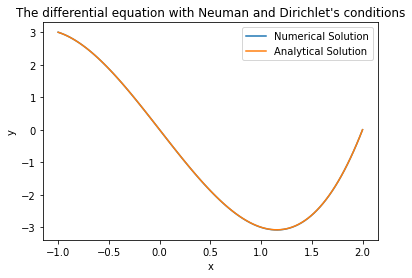
\includegraphics[scale=0.5]{img/midterm2}
    \end{center}
    \qed
\end{exampleblock} 
\end{frame}

\subsection{Điều kiện biên Robin và Neuman}

\begin{frame}
\begin{block}{Bài toán điều kiện biên Robin và Neuman}
    Tìm nghiệm của phương trình vi phân bằng phương pháp sai phân hữu hạn
    \begin{align*}
    \begin{cases}
        u''(x) - 3u'(x) + 2u(x) = 2x^3 - 9x^2 - 2x + 12, \\
        u'(-1) + u(-1) = 2, \ u'(2) = 8.
    \end{cases}
    \end{align*}
\end{block}

\begin{exampleblock}{Bài giải}
    \begin{center}\begin{tabular}{||c|c|c|c||}
    \hline
    n & Sai số tuyệt đối & Sai số tương đối & Bậc hội tụ \\
    \hline\hline
    8   & 1.8742 & 0.6151 & 2.112 \\
    16  & 0.4336 & 0.1421 & 2.028 \\
    32  & 0.1063 & 0.0345 & 2.007 \\
    64  & 0.0265 & 0.0086 & 2.002 \\
    \hline
    \end{tabular}\end{center}
\end{exampleblock}
\end{frame}

\begin{frame}
\begin{exampleblock}{Bài giải}
    \begin{center}
        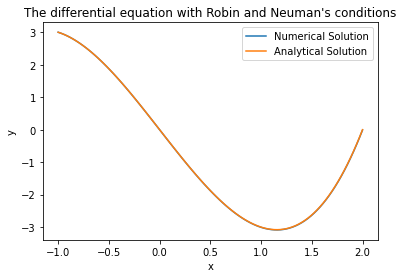
\includegraphics[scale=0.5]{img/midterm3}
    \end{center}
    \qed
\end{exampleblock} 
\end{frame}

\subsection{Điều kiện biên Robin}

\begin{frame}
\begin{block}{Bài toán điều kiện biên Robin}
    Tìm nghiệm của phương trình vi phân bằng phương pháp sai phân hữu hạn
    \begin{align*}
    \begin{cases}
        u''(x) - 3u'(x) + 2u(x) = 2x^3 - 9x^2 - 2x + 12, \\
        u'(-1) + u(-1) = 2, \ u'(2) + u(2) = 8.
    \end{cases}
    \end{align*}
\end{block}

\begin{exampleblock}{Bài giải}
    \begin{center}\begin{tabular}{||c|c|c|c||}
    \hline
    n & Sai số tuyệt đối & Sai số tương đối & Bậc hội tụ \\
    \hline\hline
    8   & 0.1391 & 0.0019 & 1.0 \\
    16  & 0.0696 & 0.0019 & 1.0 \\
    32  & 0.0348 & 0.0019 & 1.0 \\
    64  & 0.0174 & 0.0019 & 1.0 \\
    \hline
    \end{tabular}\end{center}
\end{exampleblock}
\end{frame}

\begin{frame}
\begin{exampleblock}{Bài giải}
    \begin{center}
        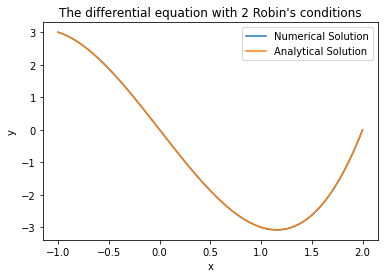
\includegraphics[scale=0.5]{img/midterm4}
    \end{center}
    \qed
\end{exampleblock} 
\end{frame}

\section{Tính nhất quán, ổn định và hội tụ của phương pháp sai phân hữu hạn}

\begin{frame}{Mục lục}
    \tableofcontents[currentsection, sections={3-4}]
\end{frame}

\subsection{Tính hội tụ}

\begin{frame}
\begin{block}{Định nghĩa Hội tụ}
    Phương pháp sai phân hữu hạn \textbf{hội tụ} khi và chỉ khi
    \begin{align*}
        \lim_{h \to \infty} \|E\| = 0.
    \end{align*}
\end{block}
\end{frame}

\subsection{Tính nhất quán}

\begin{frame}
\begin{block}{Toán tử vi phân P(d/dx)}
    Xét phương trình $u''(x) = f(x)$, khi đó $Pu = f$ tương ứng với toán tử vi phân $P$ là
    \begin{align*}
        P\left(\frac{d}{dx}\right) = \frac{d^2}{dx^2}
    \end{align*}
    Đối với phương trình $u''' + au'' + bu' + cu = f(x)$, khi đó toán tử $P$ của $Pu = f$ là
    \begin{align*}
        P\left(\frac{d}{dx}\right) = \frac{d^3}{dx^3} + a(x)\frac{d^2}{dx^2} + b(x)\frac{d}{dx} + c(x).
    \end{align*}
\end{block}
\end{frame}

\begin{frame}
\begin{block}{Toán tử sai phân hữu hạn $P_h$}
    Từ toán tử vi phân $P(d/dx)$, ta thay các đạo hàm bằng các công thức sai phân tương ứng, khi đó công thức mới là \textbf{toán tử sai phân hữu hạn} $P_h$ của toán tử $P$.
\end{block}

\begin{exampleblock}{Ví dụ}
    Xét phương trình $u''(x) = f(x)$, toán tử sai phân hữu hạn $P_h$ là
    \begin{align*}
        P_h u(x) = \frac{u(x-h) - 2u(x) + u(x+h)}{h^2}.
    \end{align*}
\end{exampleblock}
\end{frame}

\begin{frame}
\begin{block}{Định nghĩa Sai số cắt bỏ cục bộ}
    Cho $P$ và $P_h$ lần lượt là toán tử vi phân và toán tử sai phân của phương pháp sai phân hữu hạn. Khi đó \textbf{Sai số cắt bỏ cục bộ} (local truncation error) được xác định bởi
    \begin{align*}
        T(x) &= P_h(u) - P(u).
    \end{align*}
\end{block}

\begin{exampleblock}{Ví dụ}
    Xét phương trình vi phân $u''(x) = f(x)$, sai số cắt bỏ cục bộ $T$ tại điểm $x$ được tính như sau
    \begin{align*}
        T(x) &= P_h u(x) - Pu(x) \\
        &= \frac{u(x-h) - 2u(x) + u(x+h)}{h^2} - u''(x) \\
        &= \frac{u(x-h) - 2u(x) + u(x+h)}{h^2} - f(x).
    \end{align*}
\end{exampleblock}
\end{frame}

\begin{frame}
\begin{block}{Định nghĩa Nhất quán}
    Gọi $T$ là sai số cắt bỏ cục bộ của phương pháp sai phân hữu hạn. Phương pháp đạt được tính ổn định nếu
    \begin{align*}
        \lim_{h \to 0} T(x) = \lim_{h \to 0} (P_h u - Pu) = 0.
    \end{align*}
\end{block}

\begin{exampleblock}{Ví dụ}
    Xét phương trình vi phân $u''(x) = f(x)$. Ta có công thức của sai số cắt bỏ cục bộ
    \begin{align*}
        T(x) = \frac{u(x-h) - 2u(x) + u(x+h)}{h^2} - u''(x).
    \end{align*}
    Thực hiện khai triển Taylor cho từng hạng tử $u(x-h), u(x)$ và $u(x+h)$, ta được
    \begin{align*}
        T(x) = \frac{h^2}{12} u_{(4)} (x) + \ldots = O(h^2).
    \end{align*}
\end{exampleblock}
\end{frame}

\begin{frame}
\begin{exampleblock}{Ví dụ}
    Từ $\lim_{h \to 0} T(x) = \lim_{h \to 0} O(h^2) = 0$, dẫn đến tính nhất quán của phương pháp sai phân. Mặt khác
    \begin{align*}
        |T(x)| \le Ch^2, \text{ với } C = \max_{0 \le x \le 1} \left|\frac{1}{12} u^{(4)}(x)\right|
    \end{align*}
    suy ra phương pháp có bậc hội tụ là 2.
\end{exampleblock}    
\end{frame}

\subsection{Tính ổn định}

\begin{frame}
\begin{block}{Định nghĩa Ổn định}
    Cho bài toán vi phân $Pu = f$ với điều kiện biên (BVP) được giải bằng phương pháp sai phân hữu hạn, trong đó ${\bf A}$ là ma trận hệ số, ${\bf F}$ là vector cột của tác động ngoại lực $f$. Phương pháp sai phân đạt được \textbf{tính ổn định} nếu tồn tại hai hệ số $C$ và $h_0$ thoả
    \begin{align*}
        \|A^{-1}\| \le C, \text{ với mọi } 0 < h < h_0,
    \end{align*}
    chú ý $C$ và $h_0$ không phụ thuộc vào $h$.
\end{block}

\begin{exampleblock}{Định lý}
    Nếu phương pháp sai phân hữu hạn vừa có tính nhất quán vừa có tính ổn định thì hội tụ.
\end{exampleblock}
\end{frame}

\begin{frame}
\begin{block}{Bài toán}
Cho phương trình vi phân
\begin{align*}
    \begin{cases}
        u''(x) &= f(x), 0 < x < 1 \\
        u(0) &= u_a, u(1) = u_b.
    \end{cases}
\end{align*}
Chứng minh rằng phương pháp sai phân trung tâm cho phương trình thoả tính hội tụ.
\end{block}

\begin{exampleblock}{Bài giải}
    Ma trận hệ số $A$ có dạng 3 đường chéo, trong đó đường chéo chính chứa giá trị $-2/h^2$, hai đường chéo còn lại chứa giá trị $-1/h^2$. Khi đó  $A$ có các giá trị riêng là
    \begin{align*}
        \lambda_j = -\frac{2}{h^2} + \frac{2}{h^2} \cos \left(\frac{\pi j}{n}\right) = \frac{2}{h^2} \left(\cos(\pi jh) - 1\right).
    \end{align*}
\end{exampleblock}
\end{frame}

\begin{frame}
\begin{exampleblock}{Bài giải}
Do trị riêng của $A^{-1}$ là $1/\lambda_j$ và $A^{-1}$ là ma trận đối xứng, ta được
    \begin{align*}
        \|A^{-1}\|_2 &= \frac{1}{\min |\lambda_j|}
        = \frac{h^2}{2\left(\cos(\pi h)\right)} \\
        &= \frac{h^2}{2\left(1 - \frac{(\pi h)^2}{2} + \frac{(\pi h)^4}{4!} + \ldots\right)}
        < \frac{1}{\pi^2}.
    \end{align*}  
Từ bất đẳng thức $\|A^{-1}\|_\infty \le \sqrt{n-1} \|A^{-1}\|_2$, ta được
\begin{align*}
    \|E\|_\infty
    \le \|A^{-1}\|_\infty \|T\|_\infty
    \le \sqrt{n-1} \|A^{-1}\|_2 \|T\|_\infty
    \le \frac{\sqrt{n-1}}{\pi^2} Ch^2
    \le \overline{C} h^{3/2}.
\end{align*}
Do đó $\|E\|_\infty \to 0$ khi $h \to 0$, vậy phương pháp sai phân trung tâm có tính hội tụ. \qed
\end{exampleblock}
\end{frame}

\subsection{Ảnh hưởng số làm tròn}

\begin{frame}
\begin{block}{Sai số tương đối}
Việc giải phương trình vi phân bằng phương pháp sai phân hữu hạn được quy về việc giải phương trình $AU = F$, với $A$ là ma trận hệ số, $F$ là ma trận của ngoại lực. Khi đó \textbf{sai số tương đối} của phương pháp sai phân là
\begin{align*}
    \frac{\|U-u\|}{\|u\|}
    &\le \text{sai số cắt bỏ cục bộ } + \text{sai số làm tròn} \\
    &\le \|A^{-1}\|\|T\| \overline{C} g(n) \|A\|\|A^{-1}\| \epsilon.
\end{align*}
\end{block}

\begin{exampleblock}{Nhận xét}
Từ Đại số tuyến tính, ta có
\begin{align*}
    \|A\|_2 = \max |\lambda_j|
    = \frac{2}{h^2} \left(1 - \cos\left\pi(n-1)h\right)\right)
    \sim \frac{4}{h^2} = 4n^2
\end{align*}
\end{exampleblock}
\end{frame}

\begin{frame}
\begin{exampleblock}{Nhận xét}
Do tính ổn định, ta được $\|A^{-1}\| \le C'$, dẫn đến $\|A\|_2\|A^{-1}\| \sim 4n^2$. Khi đó
\begin{align*}
    \frac{\|U-u\|}{\|u\|}
    \le Ch^2 + \overline{C} g(n) \frac{1}{h^2} \epsilon
\end{align*}
Ta thấy khi $h$ giảm thì sai số cắt bỏ cục bộ giảm, nhưng sai số làm tròn lại tăng. \\

Giả sử sai số cắt bỏ cục bộ có cùng giá trị (về mặt độ lớn) với sai số làm tròn, khi đó
\begin{align*}
    h^2 \sim \frac{1}{h^2} \epsilon, \quad n \sim \frac{1}{h} = \frac{1}{\epsilon^{1/4}}.
\end{align*}
Với máy tính sử dụng số chấm động đơn (single precision), với $\epsilon = 10^{-8}$, ta được $n \approx 100$. Nếu máy tính sử dụng số chấm động kép (double precision), khi $\epsilon = 10^{-16}$, ta có $n \approx 10000$.
\end{exampleblock}
\end{frame}

\section{}

\begin{frame}
    \begin{center}
        \Huge {\bf Cảm ơn thầy và các bạn đã theo dõi!}
    \end{center}
\end{frame}

\end{document}
